%! TEX root = thesis.tex
% vim: ft=tex et sts=2 sw=2

\chapter{Introduction}

\chapterprecishere{%
  This dissertation discusses two problems that are more or less unrelated apart from having a common origin in soft matter physics.
  During the course of the discussion, we shall rely on concepts from a potpourri of fields ranging from classical and quantum mechanics to statistical mechanics to structural engineering.
  Elementary notions from differential geometry and asymptotic analysis will also play a prominent role.
  This chapter provides a whirlwind tour of the dissertation, highlighting the key results, and concludes with an organizational summary.
}

Geometrical methods are now a mainstay of all branches of modern theoretical physics.
Furthermore, vigorous research efforts in the second half of the 20th century led to the geometrization of the more classical fields of physics such as analytical mechanics~\cite{sudarshan1974,arnold1978,souder2017} and elasticity theory~\cite{marsden1994,audoly2010}.
In some sense, the unreasonable effectiveness of geometrical methods in physics (among other mathematical sciences) should come as no surprise---after all, many physical problems are best formulated mathematically in terms of configuration (or parameter) spaces that are not Euclidean.

On a less abstract level, the intrinsic shape and structure of a physical system can also play a major role in dictating its physical properties.
This is particularly true for soft, deformable materials, or ``soft matter''---the stuff of everyday things.
Indeed, mechanical pliability is often intimately connected to geometry, a fact that is appetizingly illustrated by a slice of pizza, which becomes stiff upon bending into a $\textsf{U}$ shape, thanks to Gauss's remarkable theorem.
Because soft materials are easily deformed, the presence of external perturbations such as thermal fluctuations or applied fields can have dramatic effects on their stability.
For this reason, creating materials with designer microstructure to improve their strength has become a central research theme in many disciplines, with applications cutting across several length and energy scales.

Theoretical physics abounds with exactly solvable problems and ``spherical cow'' models involving conserved quantities, rigid bodies, ideal fluids, point particles, impenetrable walls, uniform fields, and elegant linear equations.
Many of these models, however, stand in stark contrast to the fantastic haphazardness of the real world, which is messy and nonlinear, and continues to bewilder us as our experimental abilities evolve.
For this reason, many physical problems, especially those in condensed matter and materials physics---archetypal examples of the sentiment that ``more is different''~\cite{anderson1972}---can only be formulated approximately.
Furthermore, such problems often require the employment of a range of asymptotic and perturbative methods for their solution.
Such methods, perhaps fittingly, tend to be far less rigorous in comparison to the elegant logical structure usually found in other fields of mathematics.

In this dissertation we discuss two problems, at two very different length and energy scales, that have a common origin in soft matter physics.
Connecting the two problems is the basic notion that geometry, whether that of the abstract spaces describing a physical system, or its intrinsic shape and structure, plays a crucial role in dictating its properties.
Both these problems, once formulated mathematically, have sufficient complexity that makes writing down exact solutions difficult.
At the same time, both the problems are simple enough that asymptotic methods yield excellent approximate solutions, which means that we do not have to restrict ourselves to analyses of numerical experiments alone.
In the following sections, we briefly summarize the main results of this dissertation, with subsequent chapters providing more detailed descriptions.

\section{Singular frameworks and thermal fluctuations}

In the first part of the dissertation, we study the effect of thermal fluctuations on submicron mechanical frameworks.
Frameworks of similar nature have received extensive interest in recent years, with considerable attention paid to nanoscale frameworks made out of DNA origami~\cite{dunn2015,matthies2016}.
The problem is made fundamentally challenging due to the presence of singularities in the configuration spaces of these frameworks, which cause conventional approaches to break down~\cite{mannattil2022}.

\subsection{Configuration spaces}

Central to geometric mechanics is the idea that the configuration of a physical system, however complicated, can be fully described by a single point of a (usually high-dimensional) configuration space.
To illustrate this point in more familiar settings, consider, for instance, the simple pendulum in Fig.~\ref{fig:confspaces}(a).
The pendulum's configuration at any given moment is fully specified by the angle $\theta_{1}$.
Its configuration space is therefore equivalent to the circle $S^{1}$, which is a smooth manifold.
To specify the configuration of the double pendulum in Fig.~\ref{fig:confspaces}(b), on the other hand, requires two angles $\theta_{1}$ and $\theta_{2}$, and its configuration space is the torus $S^{1}\times S^{1}$.
Configuration spaces such as these, although abstract, have a one-to-one correspondence with the possible configurations that the system can be in.

To shed some more light on the above discussion and make the definitions more precise, consider a mechanical system with $n$ degrees of freedom (DOF), whose configuration at any given moment is fully described by a single configuration vector $\bm{r} \in \mathbb{R}^{n}$.
Constraints in such a system are most clearly introduced by defining a constraint map $f: \mathbb{R}^{n} \to \mathbb{R}^{m}$
that vanishes when the constraints are satisfied, with $m$ being the number of constraints introduced.
The constraint in the simple pendulum, for instance, is described by the constraint map
%
\begin{equation}
    f: \mathbb{R}^{2} \to \mathbb{R},\enspace f(r_{1}, r_{2}) = r_{1}^{2} + r_{2}^{2} - \ell^{2},
\end{equation}
%
whereas the constraint map for the double pendulum would be of the form
%
\begin{equation}
  \def\arraystretch{1}
  f: \mathbb{R}^{4} \to \mathbb{R}^{2},\enspace f(r_{1}, \ldots, r_{4}) =
\begin{pmatrix}
 r_{1}^{2} + r_{2}^{2} - \ell_{1}^{2}\\
 (r_{3} - r_{1})^{2} + (r_{4} - r_{2})^{2} - \ell_{2}^{2}
\end{pmatrix}.
\end{equation}
%
As we see from these examples, the constraint map $f$ is a general nonlinear map in the components of $\bm{r}$.
The linear approximation of $f = [f_{1}(\bm{r}), \ldots, f_{m}(\bm{r})]$ is given by the $m\times n$ Jacobian matrix $\nabla f$ whose $i\!j$th entry is $\partial_{j}f_{i}$.
With these definitions, the configuration space of a general mechanical system is the zero level set $\Omega = \{\bm{r} \in \mathbb{R}^{n} : f(\bm{r}) = 0\}$, which is the set of points where the constraints are satisfied exactly.
Standard theorems%
\footnote{These theorems are almost never explicitly invoked in classical mechanics.
However, they are implicit in the frequently used argument that a mechanical system with $n$ degrees of freedom and $m$ constraints has $(n-m)$ degrees of freedom, with the configuration space $\Omega$ parameterizable by $(n-m)$ generalized coordinates.}
ensure that $\Omega$ is a smooth $(n-m)$-dimensional manifold if the Jacobian $\nabla f$ has full rank for all points in $\Omega$.

Configuration spaces in both the above examples arose as a result of holonomic constraints imposed on a physical system.
However, the imposed holonomic constraints need not always be well-behaved.
To illustrate this point, consider a particle constrained to move on two intersecting cylinders of equal radius with mutually perpendicular axes, as illustrated in Fig.~\ref{fig:confspaces}(c).
If the particle is to obey both constraints simultaneously, it can only move on the cylinders' intersection curve, which forms the configuration space of the particle.
As we see from Fig.~\ref{fig:confspaces}(c), the curve has two singularities where it self-intersects, which prevents the configuration space from being a smooth manifold.
Mathematically, the constraints in the two-cylinder system are described by the map $f: \mathbb{R}^{3} \to \mathbb{R}^{2}$, defined by $f(x, y, z) = (x^{2} + z^{2} - 1,\, y^{2} + z^{2} - 1)$.
At singularities, such as the ones in Fig.~\ref{fig:confspaces}(c), direct computation reveals that the Jacobian $\nabla f$ drops rank.%
\footnote{Since the Jacobian is an $m\times n$ matrix, it drops rank whenever its rows---each representing a single linearized constraint---cease to become linearly independent.}
Such singularities, which arise when the constraints imposed on a system cease to be linearly independent, are not merely pathological irregularities, and they have been extensively studied in many fields, e.g., robotics and locomotion~\cite{muller2019}.
%
\begin{figure}
  \begin{center}
    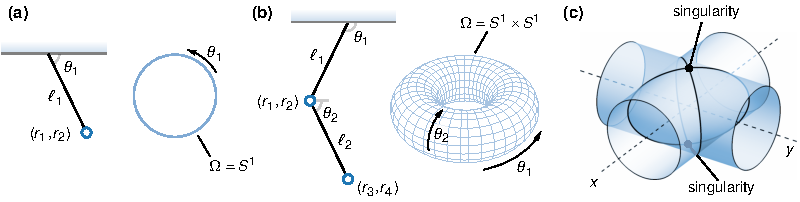
\includegraphics{intro/confspaces.pdf}
  \end{center}
  \caption{
  (a) A simple pendulum and its configuration space $\Omega = S^{1}$.
  (b) A double pendulum and its configuration space $\Omega = S^{1} \times S^{1}$.
  (c) Configuration space of a particle constrained to move on two mutually perpendicular cylinders of equal radius is the cylinders' intersection curve, which is not a smooth manifold.
  }
  \label{fig:confspaces}
\end{figure}

\subsection{Frameworks}

Soft few-body systems, composed of a small number of particles or units, interacting via short-ranged forces are commonplace in soft matter physics.
A quintessential example of such a system is a colloidal cluster, which is composed of a small number of colloidal particles with sizes typically ranging from 1~nm to 0.1~$\mu$m.
Although the particles in a colloidal cluster are held together by subtle effects of electrostatic and van der Waal forces, such details are often irrelevant if our goal is to describe the more macroscopic properties of the cluster.
To a good approximation, therefore, the interactions between the different particles are effectively described using central-force bonds connecting their centers.
Configurations of the resulting ``bond skeleton'', with each bond at its respective rest length, describe the different ground states of the cluster.
Such colloidal skeletons are an example of a mechanical framework, which is an assembly of rigid bars that connect point-like joints.
Frameworks are indeed holonomically constrained systems, not too different from the examples we have seen so far.
%
\begin{figure}
  \begin{center}
    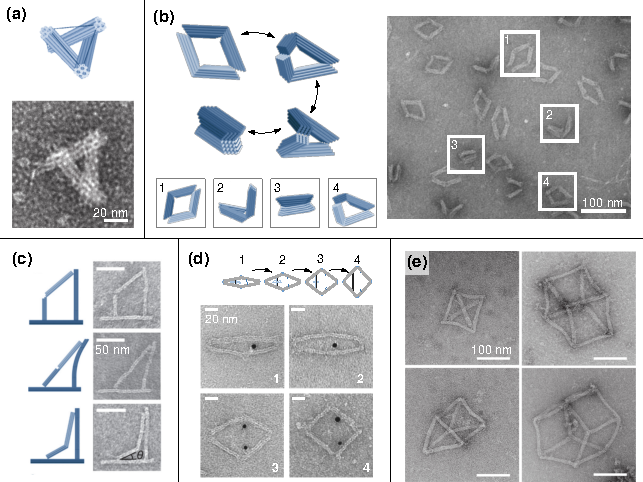
\includegraphics{intro/dna.pdf}
  \end{center}
  \caption{DNA origami has been widely used to self-assemble a variety of objects at the nanoscale.
Depicted in the figure are (a) tensegrity structures \cite{liedl2010}; (b), (c) linkage-based mechanisms \cite{marras2015,zhou2015}; (d) a rhombus-shaped nanoactuator~\cite{ke2016}; and (e) self-assembled polyhedra~\cite{iinuma2014}.}
  \label{fig:dna_origami}
\end{figure}

Apart from colloidal clusters, mechanical frameworks have been extensively used to understand a variety of mechanical structures found in viruses~\cite{hespenheide2004},
crystals~\cite{power2014} and minerals~\cite{kapko2011},
proteins~\cite{gaspar2012}, and of course,
robots and machines~\cite{farber2008,donelan2007}.
In recent years, nanoscale frameworks made out of multihelix DNA bundles (often dubbed ``DNA origami'') have received extensive interest, with applications ranging from drug delivery~\cite{zhao2019} to self-assembly~\cite{liedl2010}.
As far as more generic descriptions of thermally driven frameworks are concerned, there has been long-standing interest in the effect of thermal fluctuations on the mechanical properties of ordered and disordered lattices~\cite{zhang2016,woodhouse2018,yan2018}, and the folding of polymerized membranes~\cite{di-francesco2000,nelson2004} and polyhedral nets~\cite{shenoy2012,dodd2018,melo2020}.
There is, therefore, an arising need to understand how thermal excitations affect the physical properties of these frameworks, but only some attempts have been made so far~\cite{kallus2017,rocklin2018}.

\subsection{Free-energy landscapes}

The effect of thermal fluctuations on a physical system is often represented by its free-energy landscape in terms of a set of collective variables that provide a coarse-grained description of its slowest dynamics.
In theory~\cite{go1976,echenique2011}, one can obtain the free energy of a framework by integrating out the fast modes that are transverse to its shape space, i.e., the subset of its configuration space once rigid-body motions are removed.
Doing this, however, becomes nontrivial when the framework has shape-space singularities~\cite{zlatanov2002,liu2003,donelan2007}.
For concreteness, consider the shape space of the planar four-bar linkage~\cite{grashof1883,hartenberg1964,shimamoto2005} with freely rotating joints [Figs.~\ref{fig:4bar_collage}(a) and \ref{fig:4bar_collage}(c)].
Though this linkage has one degree of freedom up to Euclidean motions, it has two modes of deformation, one where the angle $\theta_1 = \theta_2$ and another where $\theta_1 \ne \theta_2$, meeting at two isolated singular points $(\theta_1,\theta_2) = (0,0)$ and $(\pi,\pi)$.
One generically expects the framework to be soft at these singularities, and indeed, as we see from the dashed, blue curves in Fig.~\ref{fig:4bar_collage}(b), the free energy diverges in a harmonic approximation of the elastic energy~\cite{rocklin2018}.
These divergences must be cut off by higher-order nonlinear effects, yet how this happens and to what extent remains to be understood.

In Chapters \ref{chap02} and \ref{chap03}, we develop a formalism to understand the thermal equilibration of common bar-joint frameworks that have isolated shape-space singularities.
We show that the divergent contributions to the free energy arising in the harmonic approximation to the elastic energy are suppressed by anharmonic, quartic-order corrections.
These findings show the existence of energetic free-energy barriers between configurations near the singularities and configurations farther from the singularities.
Our results are consistent with a closely related work~\cite{kallus2017,holmes-cerfon2017} on singular colloidal clusters, but allow for isolated singularities of the shape space.
We demonstrate our results using both the four-bar linkage as well as a flat, triangulated origami~\cite{chen2018}.
In addition to these two systems with one-dimensional configuration spaces, we also demonstrate the versatility of our methods using the five-bar linkage, which is a framework with a two-dimensional configuration space.
The analyses presented in these chapters have direct consequences in the design and employment of nanoscale frameworks in applications ranging from self-assembly~\cite{liedl2010} to drug delivery~\cite{zhao2019}, where relative thermodynamic stability of different configurations is of paramount importance.
%
\begin{figure}
  \begin{center}
    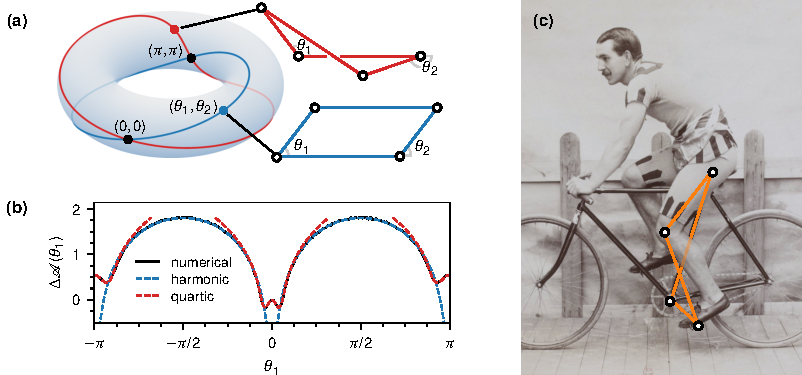
\includegraphics{intro/4bar_collage.pdf}
  \end{center}
\caption{(a) The shape space of a four-bar linkage visualized as two intersecting curves on a torus. (b) Its free energy $\mathscr{A}(\theta_{1})$ as a function of the angle $\theta_{1}$. (c) Four-bar linkage in the real world; photograph by J.~Beau, \emph{Photographie Sportive} (1898).}
  \label{fig:4bar_collage}
\end{figure}

\section{Thin structures, elastic waves, and bound states}

In the second part of this dissertation, we consider the trapping of elastic waves in thin elastic structures with spatially varying curvature profiles~\cite{mannattil2023}.
This problem was partly motivated by a fascinating acoustic phenomenon.

\subsection{Can one hear the shape of a shell?}

Take an ordinary hand saw used for cutting wood.
Clamp down the handle end of the saw using your feet and bend its tip using your dominant hand so that its overall shape is similar to the letter $\mathsf{S}$ (see Fig.~\ref{fig:saw}).
The saw is now a ``singing'' saw: bowing it or striking it with a mallet produces a sharp, sustained sound.
But how does the saw sing, and more importantly, why does it have to be shaped like an \textsf{S}?
Although the sonorousness of the common saw has been known at least since the 19th century~\cite{stuckenbruck2016}, the first scientific explanation for it was provided only in the early 90s by \citet{scott1992}.
These authors modeled the saw as a thin elastic shell with a varying curvature profile and showed that the saw's sonority is due to vibrations that get trapped around its inflection point, where the local curvature vanishes.
As trapped vibrations remain confined to the immediate vicinity of the inflection point, it reduces energy dissipation through the two ends of the saw, resulting in a sustained note.
In a very recent work, \citet{shankar2022} reported that these vibrations have a topological origin on the basis of jumps in an integer-valued invariant as we move across the inflection point.
%
\begin{figure}
  \begin{center}
    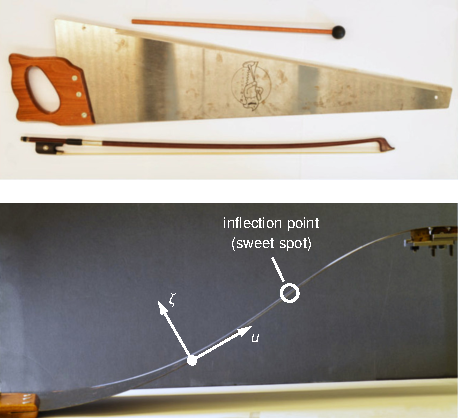
\includegraphics{intro/saw.pdf}
  \end{center}
  \caption{%
    An ordinary hand saw, when bent into the shape of the letter $\mathsf{S}$ can be played like a musical instrument using a violin's bow or a mallet.
    A sustained note is produced on bowing or hitting the saw close to its inflection point, which is called a sweet spot by saw enthusiasts.
    In most models of thin elastic structures, such as the saw here, the displacement field is broken up into a normal (e.g., $\zeta$) and tangential (e.g., $u$) component, which remain coupled if the structure is curved.
    Photographs sourced from Ref.~\cite{shankar2022}.
  }
  \label{fig:saw}
\end{figure}


Despite the efforts of the above-mentioned authors, several critical questions remain unanswered:
What kinds of waves on thin structures get trapped?
Do we really need an inflection point to observe trapped waves?  Is there a difference between the vibrational spectrum of one-dimensional and two-dimensional thin structures, i.e., rods vs. shells?
Is it possible to compute, even approximately, the shapes and frequencies of the vibrational modes?
In this dissertation, we explore these questions using a thin shell and a rod as concrete examples.

Central to understanding the trapping of waves in elastodynamic systems, such as the musical saw, is a commonplace eigenvalue problem of the form
%
\begin{equation}
  \widehat{\mathsf{D}}\psi = \omega^{2}\psi.
  \label{intro:eq:waveeq}
\end{equation}
%
Here, $\widehat{\mathsf{D}}$ is a self-adjoint linear differential operator, $\psi$ is the wave field, and $\omega$ is the frequency of vibration.
A trapped wave is a solution $\psi$ to Eq.~\eqref{intro:eq:waveeq} satisfying the prescribed boundary conditions and decaying exponentially as we approach the physical boundaries.
In physics, particularly in quantum-mechanical contexts, such solutions are called localized or bound states~\cite{ravendranadhan1989,ravendranadhan1993,ravendranadhan1994}---vocabulary that we will continue to use.

In elastodynamic problems involving thin structures, the wave field $\psi$ is almost always composed of displacements---broken up into tangential and normal components---from the neutral, undeformed configuration of the structure.
The operator $\widehat{\mathsf{D}}$, the exact nature of which is model-dependent, is a square matrix of spatial derivatives that act on $\psi$.
An uncurved elastic structure can support three basic wave types: extensional and shear waves, which respectively propagate by stretching and shearing the structure, and involve only the tangential components (e.g., $u$ in Fig.~\ref{fig:saw}); and flexural waves that propagate by bending the structure and involve only the normal component (e.g., $\zeta$ in Fig.~\ref{fig:saw}).
By contrast, if the structure is curved, the normal and tangential components remain coupled.
In this case, we can only speak of waves that are predominantly flexural or extensional or shear-like, based on which component is more dominant in magnitude.
It this curvature-mediated coupling between the various components that ultimately leads to the formation of bound states in curved structures.

\subsection{Semiclassical approximation}

The usual line of attack, when faced with an equation similar to Eq.~\eqref{intro:eq:waveeq}, is to look for plane-wave solutions of the form $\psi \sim e^{\pm i kx}$.
Such an endeavor, however, fails if the coefficients of the derivatives in $\widehat{\mathsf{D}}$ are not constants, which is the case for a thin structure with a varying curvature profile.\footnote{To be clear, as the exact form of the operator $\widehat{\mathsf{D}}$ depends on the shell or rod model we choose to work with, even when the curvature is a constant, a plain-wave solution may not be applicable.}
The semiclassical approximation or the Wentzel--Kramers--Brillouin (WKB) approximation is a widely used method to obtain approximate solutions to differential equations where these coefficients are slowly varying.
In asymptotic analysis, it is usually introduced as an approximate method to find solutions to differential equations whose highest derivative is multiplied by a small parameter~\cite{bender1978}.
A representative example from physics is the time-independent Schr\"{o}dinger equation for a particle of mass $m$ in a potential $V(x)$,
%
\begin{equation}
  \left[-\frac{\hbar^{2}}{2m}\partial_{x}^{2} + V(x)\right]\psi(x) = E\psi(x),
\end{equation}
%
where the WKB method is frequently employed to find asymptotic solutions in the limit the (reduced) Planck's constant $\hbar \to 0$.
At first glance, such a limit is perplexing and makes \emph{no} physical sense as $\hbar$ is a fundamental constant, whose value is fixed by the units we choose to work in.
In reality, the limit $\hbar \to 0$ represents the situation where the value of $\hbar$ is much smaller compared to the angular momentum scale, which is often the case with macroscopic systems described by classical physics.
It is in this context that the WKB method gets the alternative moniker of semiclassical approximation.%

Modern reformulations of the semiclassical method, based on the Weyl symbol calculus, provide unparalleled insights into the connection between classical and quantum mechanics.
Weyl calculus provides an elegant way to set up a one-to-one association between differential operators (e.g., powers of $\partial_{x}$) defined on Hilbert spaces and ordinary functions defined on a position-momentum phase space.
For instance, under the Weyl transform, the momentum operator $\hat{k} = -i\partial_{x}$ gets mapped to the momentum $k$.
Likewise, the Schr\"{o}dinger operator $\widehat{H} = -\partial_{x}^{2}/2m + V(x)$, gets mapped to the classical Hamiltonian of a point particle $H(x, k) = k^{2}/2m + V(x)$.
(For simplicity, we have suppressed factors of $\hbar$.)
To make use of Weyl calculus, it is customary to express the derivatives of a given differential operator $D(x, \partial_{x})$ in terms of $\hat{k}$ and its powers.
Then, using an integral transform, the operator can be mapped to an ordinary function---called its Weyl symbol---defined on an $x$-$k$ phase space, i.e.,
%
\begin{equation}
  \widehat{D}\left(x, \partial_{x}\right) = \widehat{D}\left(x, i\hat{k}\right) \quad\text{\small(Hilbert space)} \quad\rightleftharpoons{}\quad D\left(x, k\right) \quad\text{\small(phase space)}.
\end{equation}
%
Once the operator is in its symbol form, it can be expanded and approximated just like any other ordinary function, providing a direct path towards obtaining asymptotic solutions to wave equations.

For matrix operators that act on multicomponent wave fields, such as the one in Eq.~\eqref{intro:eq:waveeq}, the corresponding Weyl symbol $\mathsf{D}$ is called the dispersion matrix---an ordinary matrix, whose entries are functions defined on an $x$-$k$ phase space.
The eigenvalues $\lambda(x, k)$ of the dispersion matrix serve as ray Hamiltonians of the different wave types represented by Eq.~\eqref{intro:eq:waveeq}.
This leads us to the phase space representation of waves as rays that satisfy the Hamilton's equations
%
\begin{equation}
\dot{x} = \partial_{k}\lambda(x,k)
\quad\text{and}\quad
\dot{k} = -\partial_{x}\lambda(x, k).
\end{equation}
%
The advantage provided by the semiclassical approximation cannot be overstated: we have effectively reduced the wave equation to a Hamiltonian system describing point particles, a system that is much more easier to analyze.

\subsection{Bound states in thin elastic structures}

The semiclassical approximation also provides a direct route to extract the bound-state frequencies by ``quantizing'' the ray trajectories in the phase space.
As bound waves are bounded in the phase space as well, the rays corresponding to these waves appear in the form of closed orbits when visualized [see Fig.~\ref{fig:phasespace}].
Each bound orbit is associated with a wave of a specific frequency $\omega$.
The single valuedness of the wave field as we traverse the orbit requires the overall phase to be a half-integral multiple of $2\pi$, which leads to the famous Bohr--Sommerfeld quantization rule.
Additional complications and subtleties arise when the wave field has more than one component, which leads to a corrected quantization condition of the form
%
\begin{equation}
  \oint \dd{x}\,k(x) = 2\left(n + \tfrac{1}{2}\right)\pi - \left(\gamma_{\text{G}} + \gamma_{\text{NG}}\right).
\end{equation}
%
Here $\gamma_{\text{G}}$ and $\gamma_{\text{NG}}$ are extra phases that arise because of the multicomponent nature of the problem.
The phase $\gamma_{\text{G}}$ is a geometric phase~\cite{pancharatnam1956,berry1984}, which was very recently shown to be responsible for the topological protection of equatorial oceanic waves on the Earth's surface~\cite{venaille2023}.
That said, for the two example systems we study in this work, both the extra phases $\gamma_{\text{G}}$ and $\gamma_{\text{NG}}$ vanish.
Although one might expect this observation to change based on the equations we work with, it seems to be a generic result, which we expect to hold in other models of curved structures as well.

Because the extra phases vanish, the analysis becomes less cumbersome, and ultimately leads to impressive agreement between the bound-state frequencies obtained through quantization and those seen in numerical experiments.
The basic result from a combined semiclassical and numerical analysis is as follows: for the variably curved rod, which supports only extensional and flexural waves, only extensional waves form bound states; and in the case of the shell, all three wave types, i.e., flexural, extensional, and shear, exhibit bound states.
For both the shell and the rod, the bound states develop around points where the absolute curvature has a minimum.
The localization of flexural waves around the inflection point of a musical saw, which is what both \citet{scott1992} and \citet{shankar2022} restricted their attention to, is a special case of this more generic observation.
%
\begin{figure}
  \begin{center}
    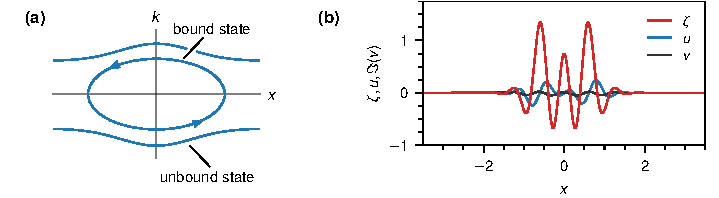
\includegraphics{figures/intro/phasespace.pdf}
  \end{center}
  \caption{(a) Phase-space representation of waves as rays, showing bound and unbound waves. (b) A predominantly flexural bound state in a uniaxially curved shell with a curvature minimum at $x = 0$ obtained by solving Eq.~\eqref{intro:eq:waveeq} numerically.
  Here $x$ is an arc-length coordinate, $\zeta$ and $u, v$ are the normal and tangential components of the displacement field, respectively; see Fig.~\ref{fig:saw} and Chapter~\ref{chap05} for more details.}
  \label{fig:phasespace}
\end{figure}
%
Many practical applications of elastic waves, from acoustic cloaking to negative refraction, rely on delicate aspects of wave localization.
The vast majority of these applications, however, require designer materials with intricate microstructures.
Being able to induce localization by a mere change of the material geometry is clearly advantageous.
For this reason, the results presented here lay the groundwork for the design of even simpler instruments capable of inducing wave localization.

\section{Organizational summary}

In Chapter~\ref{chap02} we review basic facts about frameworks, their configuration spaces, and derive asymptotic expressions for their elastic energies.
Chapter~\ref{chap03} deals with the effect that thermal fluctuations have on these frameworks, and presents a detailed calculation of the free-energy profiles for three example frameworks.
Chapters~\ref{chap04} and~\ref{chap05} are concerned with the second problem discussed in this dissertation.
The semiclassical approximation is reviewed in Chapter~\ref{chap04}, with special attention paid to multicomponent wave equations.
Chapter~\ref{chap05} makes use of the semiclassical approximation to understand the formation of bound states in thin elastic structures.
